\documentclass{beamer}
\usetheme{Frankfurt}
\usepackage[utf8]{inputenc}
\usepackage{charter}
\usepackage{graphicx}
\usepackage{amsmath}
\usepackage{amssymb}
\usepackage{listings}
\usepackage{animate}
\usepackage{bm}
\usepackage{mathtools}
\usepackage{physics}
\usepackage{caption}
\usepackage{tikz}
\usepackage{tikz-cd}
\captionsetup[figure]{labelformat=empty}
\mathtoolsset{showonlyrefs}
\beamertemplatenavigationsymbolsempty

\let\vec\bm

\usepackage{tikzit}
\documentclass{beamer}
\usetheme{Frankfurt}
\usepackage[utf8]{inputenc}
\usepackage{charter}
\usepackage{graphicx}
\usepackage{amsmath}
\usepackage{amssymb}
\usepackage{listings}
\usepackage{animate}
\usepackage{bm}
\usepackage{mathtools}
\usepackage{physics}
\usepackage{caption}
\usepackage{tikz}
\usepackage{tikz-cd}
\captionsetup[figure]{labelformat=empty}
\mathtoolsset{showonlyrefs}
\beamertemplatenavigationsymbolsempty

\let\vec\bm

\usepackage{tikzit}
\documentclass{beamer}
\usetheme{Frankfurt}
\usepackage[utf8]{inputenc}
\usepackage{charter}
\usepackage{graphicx}
\usepackage{amsmath}
\usepackage{amssymb}
\usepackage{listings}
\usepackage{animate}
\usepackage{bm}
\usepackage{mathtools}
\usepackage{physics}
\usepackage{caption}
\usepackage{tikz}
\usepackage{tikz-cd}
\captionsetup[figure]{labelformat=empty}
\mathtoolsset{showonlyrefs}
\beamertemplatenavigationsymbolsempty

\let\vec\bm

\usepackage{tikzit}
\documentclass{beamer}
\usetheme{Frankfurt}
\usepackage[utf8]{inputenc}
\usepackage{charter}
\usepackage{graphicx}
\usepackage{amsmath}
\usepackage{amssymb}
\usepackage{listings}
\usepackage{animate}
\usepackage{bm}
\usepackage{mathtools}
\usepackage{physics}
\usepackage{caption}
\usepackage{tikz}
\usepackage{tikz-cd}
\captionsetup[figure]{labelformat=empty}
\mathtoolsset{showonlyrefs}
\beamertemplatenavigationsymbolsempty

\let\vec\bm

\usepackage{tikzit}
\input{main.tikzstyles}

\pgfdeclareimage[width=\paperwidth]{titlebackground}{Images/title-slide-background.png}
\setbeamerfont{subtitle}{size=\tiny}
\setbeamertemplate{endpage}{
	\begin{picture}(0,0)
		\scalebox{1.01}{
		\put(-28.5,-163){%
			\pgfuseimage{titlebackground}
		}
		}
		\put(0,-115){%
			\begin{minipage}[b][4.5cm][t]{0.5\textwidth}
				\color{white}
				\usebeamerfont{title}
				{\textbf{Thank Your} \\ \textbf{For You Attention !}}
			\end{minipage}
		}
	\end{picture}
}
\setbeamertemplate{title page}{
	\begin{picture}(0,0)
		\scalebox{1.01}{
			\put(-28.5,-163){%
				\pgfuseimage{titlebackground}
			}
		}
		\put(0,-60){%
			\begin{minipage}[b][4.5cm][t]{0.7\textwidth}
				\color{white}
				\usebeamerfont{title}
				{\inserttitle\\[0.9cm]}
				\usebeamerfont{subtitle}
				{\insertauthor\par}
				{\insertinstitute\\[0.3cm]}
				{\insertdate}
			\end{minipage}
		}
	\end{picture}
}


%% General slide formatting %%

\definecolor{oxfordblue}{RGB}{4,30,66}
\definecolor{oxfordred}{RGB}{207,48,42}

\pgfdeclareimage[width=0.9cm]{oxfordlogo}{Images/oxford-logo.png}
\pgfdeclareimage[width=1cm]{mathslogo}{Images/mathematics-logo.png}
\pgfdeclareimage[width=1.2cm]{ngslogo}{Images/ngs-logo.png}
\pgfdeclareimage[width=1.2cm]{petsclogo}{Images/petsc-logo.png}
\pgfdeclareimage[width=1.2cm]{firedrakelogo}{Images/firedrake-logo.png}

\setbeamertemplate{headline}
{%
	\begin{picture}(0,0)
		\put(314,-50){%
			\pgfuseimage{oxfordlogo}
		}
		\put(20,-55){%
			\rule{320pt}{0.4pt}
		}
	\end{picture}
}
\def\ngshead{
	\begin{picture}(0,0)
		\put(278,0){%
			\pgfuseimage{ngslogo}
		}
		\put(-8,-5){%
			\rule{325pt}{0.4pt}
		}
	\end{picture}
}
\def\petschead{
	\begin{picture}(0,0)
		\put(278,0){%
			\pgfuseimage{petsclogo}
		}
		\put(-8,-5){%
			\rule{325pt}{0.4pt}
		}
	\end{picture}
}
\def\firedrakehead{
	\begin{picture}(0,0)
		\put(278,0){%
			\pgfuseimage{firedrakelogo}
		}
		\put(-8,-5){%
			\rule{325pt}{0.4pt}
		}
	\end{picture}
}
\setbeamertemplate{frametitle}
{%
	\begin{picture}(0,0)
		\put(-8,-20){%
			\normalsize\textbf{\color{oxfordblue}\insertframetitle}
		}
		\put(-8,-32){%
			\normalsize\textbf{\color{oxfordblue}\insertframesubtitle}
		}
	\end{picture}
}

\setbeamertemplate{footline}
{%
	\begin{picture}(0,0)
		\put(20,30){%
			\rule{320pt}{0.4pt}
		}
		\put(20,14){%
			\pgfuseimage{mathslogo}
		}
		\put(100,14){%
			\color{oxfordblue}\insertshortdate
		}
		\put(160,14){%
			\color{oxfordblue}\insertshorttitle
		}
		\put(337,14){%
			\color{oxfordblue}\insertframenumber
		}
	\end{picture}%
}
\def\footer{
	\begin{picture}(0,0)
		\put(-308,-75){%
			\rule{325pt}{0.4pt}
		}
		\put(-308,-91){%
			\pgfuseimage{mathslogo}
		}
		\put(-228,-91){%
			\color{oxfordblue}\tiny\insertshortdate
		}
		\put(-168,-91){%
			\color{oxfordblue}\tiny\insertshorttitle
		}
		\put(9,-91){%
			\color{oxfordblue}\tiny\insertframenumber
		}
	\end{picture}
}

\setbeamercolor{block title}{bg=oxfordblue!30,fg=black}
\setbeamercolor{palette primary}{bg=oxfordblue,fg=white}

\definecolor{codegreen}{rgb}{0,0.6,0}
\definecolor{codegray}{rgb}{0.5,0.5,0.5}
\definecolor{codepurple}{rgb}{0.58,0,0.82}
\definecolor{backcolour}{rgb}{0.95,0.95,0.92}

\lstdefinestyle{mystyle}{
	%backgroundcolor=\color{backcolour},   
	commentstyle=\color{codegray},
	keywordstyle=\color{oxfordblue},
	numberstyle=\tiny\color{codegray},
	stringstyle=\color{codegreen},
	basicstyle=\ttfamily\footnotesize,
	breakatwhitespace=false,         
	breaklines=true,                 
	captionpos=b,                    
	keepspaces=true,                 
	numbers=left,                    
	numbersep=5pt,                  
	showspaces=false,                
	showstringspaces=false,
	showtabs=false,                  
	tabsize=2
}
\AtBeginSection[]{
  \begin{frame}
  \vfill
  \centering
  \begin{beamercolorbox}[sep=8pt,center,shadow=true,rounded=true]{title}
    \usebeamerfont{title}\insertsectionhead\par%
  \end{beamercolorbox}
  \vfill
  \end{frame}
}

\lstset{style=mystyle}

%% Information (author, title, etc.) %%
\title[ngsPETSc]{ngsPETSc: NETGEN meets PETSc} % short title for footer
\author%
{%
	\sc{P.~E.~Farrell}*, \sc{S.~Zampini$\dag$}, \underline{\sc{U.~Zerbinati}}*\\
}
\institute%
{%
	* \textit{Mathematical Institute}\\
	\;\textit{University of Oxford}\\
	$\newline$
	$\dag$ \textit{Extreme Computing Research Center}\\
	\;\textit{King Abdullah University of Science and Technology}\\	
}

\date[\textbf{PETSc 24}]{PETSc User Meeting, 23rd of May 2024, Cologne} % short date for footer



%% Content of slides %%

\begin{document}
	\begin{frame}[plain]
		\titlepage
	\end{frame}
	\begin{frame}{Overview}
		\begin{itemize}
			\item[\color{oxfordblue}$\blacktriangleright$]
			%\item[\color{oxfordblue}$\blacktriangleright$] Reynolds robust geometric multigrid on curved meshes.
			%\item[\color{oxfordblue}$\blacktriangleright$] Easy implementation:
		\end{itemize}
		\begin{minipage}{0.58\textwidth}
			All codes are available on Github:
			\texttt{https://github.com/UZerbinati/DD28}
		\end{minipage}
		\begin{minipage}{0.3\textwidth}
			\begin{figure}
				\centering
				\includegraphics[scale=0.2]{Figures/Github.png}
			\end{figure}
		\end{minipage}
	\end{frame}
	\begin{frame}[plain]
		\frametitle{Netgen/NGSolve}
		\ngshead
		$\newline$
		$\newline$
		$\newline$
		\textbf{Netgen} is an advancing front 2D/3D-mesh generator, with many interesting features.
		\begin{itemize}
			\item[\color{oxfordblue}$\blacktriangleright$] The geometry we intend to mesh can be described by \textbf{Constructive Solid Geometry} (CSG), in particular we can use \textbf{Opencascade} to describe our geometry.
			\item[\color{oxfordblue}$\blacktriangleright$] It is able to construct \textbf{isoparametric meshes} reppresentation, which conform to the geometry.
			\item[\color{oxfordblue}$\blacktriangleright$] A wide variety of mesh splits are available also for curved geometries, such as Alfeld splits and Powell-Sabin splits. 
			\item[\color{oxfordblue}$\blacktriangleright$] High flexibility in the mesh generation and mesh refinement.
		\end{itemize}
	\end{frame}
	\begin{frame}[plain]
		\frametitle{Netgen/NGSolve}
		\ngshead
		$\newline$
		$\newline$
		$\newline$
		\textbf{NGSolve} is a high-performance multiphysics finite element software with an extremely flexible Python interface.
		\begin{itemize}
			\item[\color{oxfordblue}$\blacktriangleright$] Wide range of finite elements available, including and not limited to hierarchical $H^1$ elements, $H(div)$ Raviart-Thomas and Brezzi-Douglas-Marini elements, and $H(curl)$ Nedelec elements.
			\item[\color{oxfordblue}$\blacktriangleright$] The variational formulation can be easily defined using an analogous language to the unified form language (UFL).
			\item[\color{oxfordblue}$\blacktriangleright$] Many extensions are available, including \textbf{ngsxfem} for unfitted finite element discretizations, \textbf{ngsTreffetz} for Treffetz methods and \textbf{ngsTents} for spacetime tents schemes.
		\end{itemize}
	\end{frame}
	\begin{frame}
		\frametitle{ngsPETSc -- NETGEN/NGSolve}
		$\newline$
		\textbf{ngsPETSc} is an interface between NETGEN/NGSolve and \textbf{PETSc}. In particular, \textbf{ngsPETSc} provides new capabilities to \textbf{NETGEN}/\textbf{NGSolve} such as:
		$\newline$
		\begin{itemize}
			\item[\color{oxfordblue}$\blacktriangleright$] Access to all linear solver capabilities of \textbf{KSP}.
			\item[\color{oxfordblue}$\blacktriangleright$] Access to all preconditioning capabilities of \textbf{PC}.
			\item[\color{oxfordblue}$\blacktriangleright$] Access to all non-linear solver capabilities of \textbf{SNES}.
			\item[\color{oxfordblue}$\blacktriangleright$] Access to all mesh refinement capabilities of \textbf{DMPLEX}.
		\end{itemize}
	\end{frame}
	\section{\textbf{PETSc KSP}}
	\begin{frame}[plain]
		\frametitle{An NGsolve Example}
		\ngshead
		$\newline$
		\lstinputlisting[language=Python, firstline=12, lastline=26]{../examples/ngs/ksp_poisson.py.rst}
	\end{frame}
	\begin{frame}[plain]
		\frametitle{PETSc KSP -- Direct solve with MUMPS }
		\ngshead
		$\newline$
		$\newline$
		\color{oxfordblue}$\blacktriangleright$ We can perform a direct solve using MUMPS.
		\begin{columns}[T]
			\begin{column}{0.7\textwidth}
				\lstinputlisting[language=Python, firstline=37, lastline=45]{../examples/ngs/ksp_poisson.py.rst}
			\end{column}
			\begin{column}{0.3\textwidth}
				\begin{figure}
					\centering
					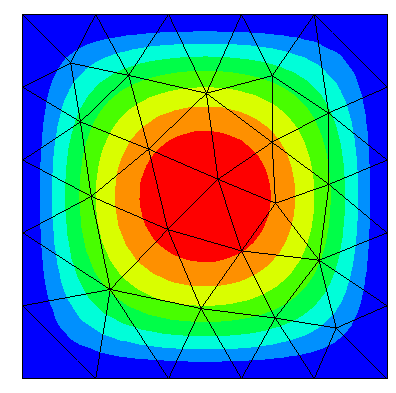
\includegraphics[scale=0.3]{../figures/mumps.png}
					\caption*{\tiny{Solution of Poisson problem computed with MUMPS}}
				\end{figure}
			\end{column}
		\end{columns}
	\end{frame}
	\begin{frame}[plain]
		\frametitle{PETSc KSP -- Iterative Jacobi method}
		\ngshead
		$\newline$
		$\newline$
		\color{oxfordblue}$\blacktriangleright$ We can use a wide variety of iterative solvers, for example, the Jacobi method, i.e.
		\begin{equation}
			x^{(k+1)} = D^{-1}(b - (A - D)x^{(k)}).
		\end{equation}
		\lstinputlisting[language=Python, firstline=52, lastline=58]{../examples/ngs/ksp_poisson.py.rst}
		$\newline$
		\color{oxfordblue}$\blacktriangleright$ Analogously we can implement the Gauss-Seidel method. 
	\end{frame}
	\begin{frame}[plain]
		\frametitle{PETSc KSP -- Geometric Algebraic MultiGrid (GAMG)}
		\ngshead
		$\newline$
		$\newline$
		$\newline$
		\color{oxfordblue}$\blacktriangleright$ Inside of a classical iterative method such as conjugate gradient, we can play with different preconditioners such as PETSc GAMG.
		$\newline$
		\lstinputlisting[language=Python, firstline=61, lastline=64]{../examples/ngs/ksp_poisson.py.rst}
		$\newline$
		\color{oxfordblue}$\blacktriangleright$ As we will see in a moment we have a wide variety of preconditioners available, such as: \textbf{Hypre (GAMG)}, \textbf{BDDC}, \textbf{...} 
	\end{frame}
	%\begin{frame}[plain]
	%	\firedrakehead
	%	$\newline$
	%	$\newline$
	%	\textbf{Firedrake} is an automated system for the solution of partial differential equations using the finite element method (FEM).
	%	$\newline$
	%	$\newline$
	%		\begin{itemize}
	%			\item[\color{oxfordblue}$\blacktriangleright$] Variational formulation can be easily defined using the \textbf{UFL} language.
	%			\item[\color{oxfordblue}$\blacktriangleright$] Wide class of finite elements are available, including $H(div)$, $H(curl)$, $H^1$ and $H^2$.
	%			\item[\color{oxfordblue}$\blacktriangleright$] Provides access to \textbf{PETSc} linear solvers and non-linear solvers.
	%		\end{itemize}
	%\end{frame}
	%\begin{frame}
	%	\frametitle{ngsPETSc -- Firedrake}
	%	$\newline$
	%	\textbf{ngsPETSc} provides new capabilities to \textbf{Firedrake} such as:
	%	$\newline$
	%	\begin{itemize}
	%		\item[\color{oxfordblue}$\blacktriangleright$] Access to all Netgen generated linear meshes and high order meshes.
	%		\item[\color{oxfordblue}$\blacktriangleright$] Splits for macro elements, such as Alfeld splits and Powell-Sabin splits (even on curved geometries).
	%		\item[\color{oxfordblue}$\blacktriangleright$] Adaptive mesh refinement capabilities, that conform to the geometry.
	%		\item[\color{oxfordblue}$\blacktriangleright$] High order mesh hierarchies for multigrid solvers. 
	%	\end{itemize}
	%\end{frame}
	%\begin{frame}
	%	\frametitle{Firedrake' 24}
	%	$\newline$
	%	Join us at the Firedrake user and developer workshop that will be held between 16-18 September 2024 at the University of Oxford.
	%\end{frame}
\end{document}


\pgfdeclareimage[width=\paperwidth]{titlebackground}{Images/title-slide-background.png}
\setbeamerfont{subtitle}{size=\tiny}
\setbeamertemplate{endpage}{
	\begin{picture}(0,0)
		\scalebox{1.01}{
		\put(-28.5,-163){%
			\pgfuseimage{titlebackground}
		}
		}
		\put(0,-115){%
			\begin{minipage}[b][4.5cm][t]{0.5\textwidth}
				\color{white}
				\usebeamerfont{title}
				{\textbf{Thank Your} \\ \textbf{For You Attention !}}
			\end{minipage}
		}
	\end{picture}
}
\setbeamertemplate{title page}{
	\begin{picture}(0,0)
		\scalebox{1.01}{
			\put(-28.5,-163){%
				\pgfuseimage{titlebackground}
			}
		}
		\put(0,-60){%
			\begin{minipage}[b][4.5cm][t]{0.7\textwidth}
				\color{white}
				\usebeamerfont{title}
				{\inserttitle\\[0.9cm]}
				\usebeamerfont{subtitle}
				{\insertauthor\par}
				{\insertinstitute\\[0.3cm]}
				{\insertdate}
			\end{minipage}
		}
	\end{picture}
}


%% General slide formatting %%

\definecolor{oxfordblue}{RGB}{4,30,66}
\definecolor{oxfordred}{RGB}{207,48,42}

\pgfdeclareimage[width=0.9cm]{oxfordlogo}{Images/oxford-logo.png}
\pgfdeclareimage[width=1cm]{mathslogo}{Images/mathematics-logo.png}
\pgfdeclareimage[width=1.2cm]{ngslogo}{Images/ngs-logo.png}
\pgfdeclareimage[width=1.2cm]{petsclogo}{Images/petsc-logo.png}
\pgfdeclareimage[width=1.2cm]{firedrakelogo}{Images/firedrake-logo.png}

\setbeamertemplate{headline}
{%
	\begin{picture}(0,0)
		\put(314,-50){%
			\pgfuseimage{oxfordlogo}
		}
		\put(20,-55){%
			\rule{320pt}{0.4pt}
		}
	\end{picture}
}
\def\ngshead{
	\begin{picture}(0,0)
		\put(278,0){%
			\pgfuseimage{ngslogo}
		}
		\put(-8,-5){%
			\rule{325pt}{0.4pt}
		}
	\end{picture}
}
\def\petschead{
	\begin{picture}(0,0)
		\put(278,0){%
			\pgfuseimage{petsclogo}
		}
		\put(-8,-5){%
			\rule{325pt}{0.4pt}
		}
	\end{picture}
}
\def\firedrakehead{
	\begin{picture}(0,0)
		\put(278,0){%
			\pgfuseimage{firedrakelogo}
		}
		\put(-8,-5){%
			\rule{325pt}{0.4pt}
		}
	\end{picture}
}
\setbeamertemplate{frametitle}
{%
	\begin{picture}(0,0)
		\put(-8,-20){%
			\normalsize\textbf{\color{oxfordblue}\insertframetitle}
		}
		\put(-8,-32){%
			\normalsize\textbf{\color{oxfordblue}\insertframesubtitle}
		}
	\end{picture}
}

\setbeamertemplate{footline}
{%
	\begin{picture}(0,0)
		\put(20,30){%
			\rule{320pt}{0.4pt}
		}
		\put(20,14){%
			\pgfuseimage{mathslogo}
		}
		\put(100,14){%
			\color{oxfordblue}\insertshortdate
		}
		\put(160,14){%
			\color{oxfordblue}\insertshorttitle
		}
		\put(337,14){%
			\color{oxfordblue}\insertframenumber
		}
	\end{picture}%
}
\def\footer{
	\begin{picture}(0,0)
		\put(-308,-75){%
			\rule{325pt}{0.4pt}
		}
		\put(-308,-91){%
			\pgfuseimage{mathslogo}
		}
		\put(-228,-91){%
			\color{oxfordblue}\tiny\insertshortdate
		}
		\put(-168,-91){%
			\color{oxfordblue}\tiny\insertshorttitle
		}
		\put(9,-91){%
			\color{oxfordblue}\tiny\insertframenumber
		}
	\end{picture}
}

\setbeamercolor{block title}{bg=oxfordblue!30,fg=black}
\setbeamercolor{palette primary}{bg=oxfordblue,fg=white}

\definecolor{codegreen}{rgb}{0,0.6,0}
\definecolor{codegray}{rgb}{0.5,0.5,0.5}
\definecolor{codepurple}{rgb}{0.58,0,0.82}
\definecolor{backcolour}{rgb}{0.95,0.95,0.92}

\lstdefinestyle{mystyle}{
	%backgroundcolor=\color{backcolour},   
	commentstyle=\color{codegray},
	keywordstyle=\color{oxfordblue},
	numberstyle=\tiny\color{codegray},
	stringstyle=\color{codegreen},
	basicstyle=\ttfamily\footnotesize,
	breakatwhitespace=false,         
	breaklines=true,                 
	captionpos=b,                    
	keepspaces=true,                 
	numbers=left,                    
	numbersep=5pt,                  
	showspaces=false,                
	showstringspaces=false,
	showtabs=false,                  
	tabsize=2
}
\AtBeginSection[]{
  \begin{frame}
  \vfill
  \centering
  \begin{beamercolorbox}[sep=8pt,center,shadow=true,rounded=true]{title}
    \usebeamerfont{title}\insertsectionhead\par%
  \end{beamercolorbox}
  \vfill
  \end{frame}
}

\lstset{style=mystyle}

%% Information (author, title, etc.) %%
\title[ngsPETSc]{ngsPETSc: NETGEN meets PETSc} % short title for footer
\author%
{%
	\sc{P.~E.~Farrell}*, \sc{S.~Zampini$\dag$}, \underline{\sc{U.~Zerbinati}}*\\
}
\institute%
{%
	* \textit{Mathematical Institute}\\
	\;\textit{University of Oxford}\\
	$\newline$
	$\dag$ \textit{Extreme Computing Research Center}\\
	\;\textit{King Abdullah University of Science and Technology}\\	
}

\date[\textbf{PETSc 24}]{PETSc User Meeting, 23rd of May 2024, Cologne} % short date for footer



%% Content of slides %%

\begin{document}
	\begin{frame}[plain]
		\titlepage
	\end{frame}
	\begin{frame}{Overview}
		\begin{itemize}
			\item[\color{oxfordblue}$\blacktriangleright$]
			%\item[\color{oxfordblue}$\blacktriangleright$] Reynolds robust geometric multigrid on curved meshes.
			%\item[\color{oxfordblue}$\blacktriangleright$] Easy implementation:
		\end{itemize}
		\begin{minipage}{0.58\textwidth}
			All codes are available on Github:
			\texttt{https://github.com/UZerbinati/DD28}
		\end{minipage}
		\begin{minipage}{0.3\textwidth}
			\begin{figure}
				\centering
				\includegraphics[scale=0.2]{Figures/Github.png}
			\end{figure}
		\end{minipage}
	\end{frame}
	\begin{frame}[plain]
		\frametitle{Netgen/NGSolve}
		\ngshead
		$\newline$
		$\newline$
		$\newline$
		\textbf{Netgen} is an advancing front 2D/3D-mesh generator, with many interesting features.
		\begin{itemize}
			\item[\color{oxfordblue}$\blacktriangleright$] The geometry we intend to mesh can be described by \textbf{Constructive Solid Geometry} (CSG), in particular we can use \textbf{Opencascade} to describe our geometry.
			\item[\color{oxfordblue}$\blacktriangleright$] It is able to construct \textbf{isoparametric meshes} reppresentation, which conform to the geometry.
			\item[\color{oxfordblue}$\blacktriangleright$] A wide variety of mesh splits are available also for curved geometries, such as Alfeld splits and Powell-Sabin splits. 
			\item[\color{oxfordblue}$\blacktriangleright$] High flexibility in the mesh generation and mesh refinement.
		\end{itemize}
	\end{frame}
	\begin{frame}[plain]
		\frametitle{Netgen/NGSolve}
		\ngshead
		$\newline$
		$\newline$
		$\newline$
		\textbf{NGSolve} is a high-performance multiphysics finite element software with an extremely flexible Python interface.
		\begin{itemize}
			\item[\color{oxfordblue}$\blacktriangleright$] Wide range of finite elements available, including and not limited to hierarchical $H^1$ elements, $H(div)$ Raviart-Thomas and Brezzi-Douglas-Marini elements, and $H(curl)$ Nedelec elements.
			\item[\color{oxfordblue}$\blacktriangleright$] The variational formulation can be easily defined using an analogous language to the unified form language (UFL).
			\item[\color{oxfordblue}$\blacktriangleright$] Many extensions are available, including \textbf{ngsxfem} for unfitted finite element discretizations, \textbf{ngsTreffetz} for Treffetz methods and \textbf{ngsTents} for spacetime tents schemes.
		\end{itemize}
	\end{frame}
	\begin{frame}
		\frametitle{ngsPETSc -- NETGEN/NGSolve}
		$\newline$
		\textbf{ngsPETSc} is an interface between NETGEN/NGSolve and \textbf{PETSc}. In particular, \textbf{ngsPETSc} provides new capabilities to \textbf{NETGEN}/\textbf{NGSolve} such as:
		$\newline$
		\begin{itemize}
			\item[\color{oxfordblue}$\blacktriangleright$] Access to all linear solver capabilities of \textbf{KSP}.
			\item[\color{oxfordblue}$\blacktriangleright$] Access to all preconditioning capabilities of \textbf{PC}.
			\item[\color{oxfordblue}$\blacktriangleright$] Access to all non-linear solver capabilities of \textbf{SNES}.
			\item[\color{oxfordblue}$\blacktriangleright$] Access to all mesh refinement capabilities of \textbf{DMPLEX}.
		\end{itemize}
	\end{frame}
	\section{\textbf{PETSc KSP}}
	\begin{frame}[plain]
		\frametitle{An NGsolve Example}
		\ngshead
		$\newline$
		\lstinputlisting[language=Python, firstline=12, lastline=26]{../examples/ngs/ksp_poisson.py.rst}
	\end{frame}
	\begin{frame}[plain]
		\frametitle{PETSc KSP -- Direct solve with MUMPS }
		\ngshead
		$\newline$
		$\newline$
		\color{oxfordblue}$\blacktriangleright$ We can perform a direct solve using MUMPS.
		\begin{columns}[T]
			\begin{column}{0.7\textwidth}
				\lstinputlisting[language=Python, firstline=37, lastline=45]{../examples/ngs/ksp_poisson.py.rst}
			\end{column}
			\begin{column}{0.3\textwidth}
				\begin{figure}
					\centering
					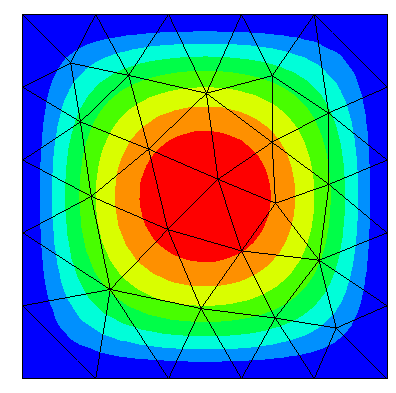
\includegraphics[scale=0.3]{../figures/mumps.png}
					\caption*{\tiny{Solution of Poisson problem computed with MUMPS}}
				\end{figure}
			\end{column}
		\end{columns}
	\end{frame}
	\begin{frame}[plain]
		\frametitle{PETSc KSP -- Iterative Jacobi method}
		\ngshead
		$\newline$
		$\newline$
		\color{oxfordblue}$\blacktriangleright$ We can use a wide variety of iterative solvers, for example, the Jacobi method, i.e.
		\begin{equation}
			x^{(k+1)} = D^{-1}(b - (A - D)x^{(k)}).
		\end{equation}
		\lstinputlisting[language=Python, firstline=52, lastline=58]{../examples/ngs/ksp_poisson.py.rst}
		$\newline$
		\color{oxfordblue}$\blacktriangleright$ Analogously we can implement the Gauss-Seidel method. 
	\end{frame}
	\begin{frame}[plain]
		\frametitle{PETSc KSP -- Geometric Algebraic MultiGrid (GAMG)}
		\ngshead
		$\newline$
		$\newline$
		$\newline$
		\color{oxfordblue}$\blacktriangleright$ Inside of a classical iterative method such as conjugate gradient, we can play with different preconditioners such as PETSc GAMG.
		$\newline$
		\lstinputlisting[language=Python, firstline=61, lastline=64]{../examples/ngs/ksp_poisson.py.rst}
		$\newline$
		\color{oxfordblue}$\blacktriangleright$ As we will see in a moment we have a wide variety of preconditioners available, such as: \textbf{Hypre (GAMG)}, \textbf{BDDC}, \textbf{...} 
	\end{frame}
	%\begin{frame}[plain]
	%	\firedrakehead
	%	$\newline$
	%	$\newline$
	%	\textbf{Firedrake} is an automated system for the solution of partial differential equations using the finite element method (FEM).
	%	$\newline$
	%	$\newline$
	%		\begin{itemize}
	%			\item[\color{oxfordblue}$\blacktriangleright$] Variational formulation can be easily defined using the \textbf{UFL} language.
	%			\item[\color{oxfordblue}$\blacktriangleright$] Wide class of finite elements are available, including $H(div)$, $H(curl)$, $H^1$ and $H^2$.
	%			\item[\color{oxfordblue}$\blacktriangleright$] Provides access to \textbf{PETSc} linear solvers and non-linear solvers.
	%		\end{itemize}
	%\end{frame}
	%\begin{frame}
	%	\frametitle{ngsPETSc -- Firedrake}
	%	$\newline$
	%	\textbf{ngsPETSc} provides new capabilities to \textbf{Firedrake} such as:
	%	$\newline$
	%	\begin{itemize}
	%		\item[\color{oxfordblue}$\blacktriangleright$] Access to all Netgen generated linear meshes and high order meshes.
	%		\item[\color{oxfordblue}$\blacktriangleright$] Splits for macro elements, such as Alfeld splits and Powell-Sabin splits (even on curved geometries).
	%		\item[\color{oxfordblue}$\blacktriangleright$] Adaptive mesh refinement capabilities, that conform to the geometry.
	%		\item[\color{oxfordblue}$\blacktriangleright$] High order mesh hierarchies for multigrid solvers. 
	%	\end{itemize}
	%\end{frame}
	%\begin{frame}
	%	\frametitle{Firedrake' 24}
	%	$\newline$
	%	Join us at the Firedrake user and developer workshop that will be held between 16-18 September 2024 at the University of Oxford.
	%\end{frame}
\end{document}


\pgfdeclareimage[width=\paperwidth]{titlebackground}{Images/title-slide-background.png}
\setbeamerfont{subtitle}{size=\tiny}
\setbeamertemplate{endpage}{
	\begin{picture}(0,0)
		\scalebox{1.01}{
		\put(-28.5,-163){%
			\pgfuseimage{titlebackground}
		}
		}
		\put(0,-115){%
			\begin{minipage}[b][4.5cm][t]{0.5\textwidth}
				\color{white}
				\usebeamerfont{title}
				{\textbf{Thank Your} \\ \textbf{For You Attention !}}
			\end{minipage}
		}
	\end{picture}
}
\setbeamertemplate{title page}{
	\begin{picture}(0,0)
		\scalebox{1.01}{
			\put(-28.5,-163){%
				\pgfuseimage{titlebackground}
			}
		}
		\put(0,-60){%
			\begin{minipage}[b][4.5cm][t]{0.7\textwidth}
				\color{white}
				\usebeamerfont{title}
				{\inserttitle\\[0.9cm]}
				\usebeamerfont{subtitle}
				{\insertauthor\par}
				{\insertinstitute\\[0.3cm]}
				{\insertdate}
			\end{minipage}
		}
	\end{picture}
}


%% General slide formatting %%

\definecolor{oxfordblue}{RGB}{4,30,66}
\definecolor{oxfordred}{RGB}{207,48,42}

\pgfdeclareimage[width=0.9cm]{oxfordlogo}{Images/oxford-logo.png}
\pgfdeclareimage[width=1cm]{mathslogo}{Images/mathematics-logo.png}
\pgfdeclareimage[width=1.2cm]{ngslogo}{Images/ngs-logo.png}
\pgfdeclareimage[width=1.2cm]{petsclogo}{Images/petsc-logo.png}
\pgfdeclareimage[width=1.2cm]{firedrakelogo}{Images/firedrake-logo.png}

\setbeamertemplate{headline}
{%
	\begin{picture}(0,0)
		\put(314,-50){%
			\pgfuseimage{oxfordlogo}
		}
		\put(20,-55){%
			\rule{320pt}{0.4pt}
		}
	\end{picture}
}
\def\ngshead{
	\begin{picture}(0,0)
		\put(278,0){%
			\pgfuseimage{ngslogo}
		}
		\put(-8,-5){%
			\rule{325pt}{0.4pt}
		}
	\end{picture}
}
\def\petschead{
	\begin{picture}(0,0)
		\put(278,0){%
			\pgfuseimage{petsclogo}
		}
		\put(-8,-5){%
			\rule{325pt}{0.4pt}
		}
	\end{picture}
}
\def\firedrakehead{
	\begin{picture}(0,0)
		\put(278,0){%
			\pgfuseimage{firedrakelogo}
		}
		\put(-8,-5){%
			\rule{325pt}{0.4pt}
		}
	\end{picture}
}
\setbeamertemplate{frametitle}
{%
	\begin{picture}(0,0)
		\put(-8,-20){%
			\normalsize\textbf{\color{oxfordblue}\insertframetitle}
		}
		\put(-8,-32){%
			\normalsize\textbf{\color{oxfordblue}\insertframesubtitle}
		}
	\end{picture}
}

\setbeamertemplate{footline}
{%
	\begin{picture}(0,0)
		\put(20,30){%
			\rule{320pt}{0.4pt}
		}
		\put(20,14){%
			\pgfuseimage{mathslogo}
		}
		\put(100,14){%
			\color{oxfordblue}\insertshortdate
		}
		\put(160,14){%
			\color{oxfordblue}\insertshorttitle
		}
		\put(337,14){%
			\color{oxfordblue}\insertframenumber
		}
	\end{picture}%
}
\def\footer{
	\begin{picture}(0,0)
		\put(-308,-75){%
			\rule{325pt}{0.4pt}
		}
		\put(-308,-91){%
			\pgfuseimage{mathslogo}
		}
		\put(-228,-91){%
			\color{oxfordblue}\tiny\insertshortdate
		}
		\put(-168,-91){%
			\color{oxfordblue}\tiny\insertshorttitle
		}
		\put(9,-91){%
			\color{oxfordblue}\tiny\insertframenumber
		}
	\end{picture}
}

\setbeamercolor{block title}{bg=oxfordblue!30,fg=black}
\setbeamercolor{palette primary}{bg=oxfordblue,fg=white}

\definecolor{codegreen}{rgb}{0,0.6,0}
\definecolor{codegray}{rgb}{0.5,0.5,0.5}
\definecolor{codepurple}{rgb}{0.58,0,0.82}
\definecolor{backcolour}{rgb}{0.95,0.95,0.92}

\lstdefinestyle{mystyle}{
	%backgroundcolor=\color{backcolour},   
	commentstyle=\color{codegray},
	keywordstyle=\color{oxfordblue},
	numberstyle=\tiny\color{codegray},
	stringstyle=\color{codegreen},
	basicstyle=\ttfamily\footnotesize,
	breakatwhitespace=false,         
	breaklines=true,                 
	captionpos=b,                    
	keepspaces=true,                 
	numbers=left,                    
	numbersep=5pt,                  
	showspaces=false,                
	showstringspaces=false,
	showtabs=false,                  
	tabsize=2
}
\AtBeginSection[]{
  \begin{frame}
  \vfill
  \centering
  \begin{beamercolorbox}[sep=8pt,center,shadow=true,rounded=true]{title}
    \usebeamerfont{title}\insertsectionhead\par%
  \end{beamercolorbox}
  \vfill
  \end{frame}
}

\lstset{style=mystyle}

%% Information (author, title, etc.) %%
\title[ngsPETSc]{ngsPETSc: NETGEN meets PETSc} % short title for footer
\author%
{%
	\sc{P.~E.~Farrell}*, \sc{S.~Zampini$\dag$}, \underline{\sc{U.~Zerbinati}}*\\
}
\institute%
{%
	* \textit{Mathematical Institute}\\
	\;\textit{University of Oxford}\\
	$\newline$
	$\dag$ \textit{Extreme Computing Research Center}\\
	\;\textit{King Abdullah University of Science and Technology}\\	
}

\date[\textbf{PETSc 24}]{PETSc User Meeting, 23rd of May 2024, Cologne} % short date for footer



%% Content of slides %%

\begin{document}
	\begin{frame}[plain]
		\titlepage
	\end{frame}
	\begin{frame}{Overview}
		\begin{itemize}
			\item[\color{oxfordblue}$\blacktriangleright$]
			%\item[\color{oxfordblue}$\blacktriangleright$] Reynolds robust geometric multigrid on curved meshes.
			%\item[\color{oxfordblue}$\blacktriangleright$] Easy implementation:
		\end{itemize}
		\begin{minipage}{0.58\textwidth}
			All codes are available on Github:
			\texttt{https://github.com/UZerbinati/DD28}
		\end{minipage}
		\begin{minipage}{0.3\textwidth}
			\begin{figure}
				\centering
				\includegraphics[scale=0.2]{Figures/Github.png}
			\end{figure}
		\end{minipage}
	\end{frame}
	\begin{frame}[plain]
		\frametitle{Netgen/NGSolve}
		\ngshead
		$\newline$
		$\newline$
		$\newline$
		\textbf{Netgen} is an advancing front 2D/3D-mesh generator, with many interesting features.
		\begin{itemize}
			\item[\color{oxfordblue}$\blacktriangleright$] The geometry we intend to mesh can be described by \textbf{Constructive Solid Geometry} (CSG), in particular we can use \textbf{Opencascade} to describe our geometry.
			\item[\color{oxfordblue}$\blacktriangleright$] It is able to construct \textbf{isoparametric meshes} reppresentation, which conform to the geometry.
			\item[\color{oxfordblue}$\blacktriangleright$] A wide variety of mesh splits are available also for curved geometries, such as Alfeld splits and Powell-Sabin splits. 
			\item[\color{oxfordblue}$\blacktriangleright$] High flexibility in the mesh generation and mesh refinement.
		\end{itemize}
	\end{frame}
	\begin{frame}[plain]
		\frametitle{Netgen/NGSolve}
		\ngshead
		$\newline$
		$\newline$
		$\newline$
		\textbf{NGSolve} is a high-performance multiphysics finite element software with an extremely flexible Python interface.
		\begin{itemize}
			\item[\color{oxfordblue}$\blacktriangleright$] Wide range of finite elements available, including and not limited to hierarchical $H^1$ elements, $H(div)$ Raviart-Thomas and Brezzi-Douglas-Marini elements, and $H(curl)$ Nedelec elements.
			\item[\color{oxfordblue}$\blacktriangleright$] The variational formulation can be easily defined using an analogous language to the unified form language (UFL).
			\item[\color{oxfordblue}$\blacktriangleright$] Many extensions are available, including \textbf{ngsxfem} for unfitted finite element discretizations, \textbf{ngsTreffetz} for Treffetz methods and \textbf{ngsTents} for spacetime tents schemes.
		\end{itemize}
	\end{frame}
	\begin{frame}
		\frametitle{ngsPETSc -- NETGEN/NGSolve}
		$\newline$
		\textbf{ngsPETSc} is an interface between NETGEN/NGSolve and \textbf{PETSc}. In particular, \textbf{ngsPETSc} provides new capabilities to \textbf{NETGEN}/\textbf{NGSolve} such as:
		$\newline$
		\begin{itemize}
			\item[\color{oxfordblue}$\blacktriangleright$] Access to all linear solver capabilities of \textbf{KSP}.
			\item[\color{oxfordblue}$\blacktriangleright$] Access to all preconditioning capabilities of \textbf{PC}.
			\item[\color{oxfordblue}$\blacktriangleright$] Access to all non-linear solver capabilities of \textbf{SNES}.
			\item[\color{oxfordblue}$\blacktriangleright$] Access to all mesh refinement capabilities of \textbf{DMPLEX}.
		\end{itemize}
	\end{frame}
	\section{\textbf{PETSc KSP}}
	\begin{frame}[plain]
		\frametitle{An NGsolve Example}
		\ngshead
		$\newline$
		\lstinputlisting[language=Python, firstline=12, lastline=26]{../examples/ngs/ksp_poisson.py.rst}
	\end{frame}
	\begin{frame}[plain]
		\frametitle{PETSc KSP -- Direct solve with MUMPS }
		\ngshead
		$\newline$
		$\newline$
		\color{oxfordblue}$\blacktriangleright$ We can perform a direct solve using MUMPS.
		\begin{columns}[T]
			\begin{column}{0.7\textwidth}
				\lstinputlisting[language=Python, firstline=37, lastline=45]{../examples/ngs/ksp_poisson.py.rst}
			\end{column}
			\begin{column}{0.3\textwidth}
				\begin{figure}
					\centering
					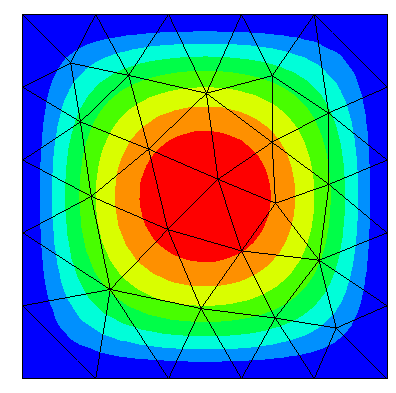
\includegraphics[scale=0.3]{../figures/mumps.png}
					\caption*{\tiny{Solution of Poisson problem computed with MUMPS}}
				\end{figure}
			\end{column}
		\end{columns}
	\end{frame}
	\begin{frame}[plain]
		\frametitle{PETSc KSP -- Iterative Jacobi method}
		\ngshead
		$\newline$
		$\newline$
		\color{oxfordblue}$\blacktriangleright$ We can use a wide variety of iterative solvers, for example, the Jacobi method, i.e.
		\begin{equation}
			x^{(k+1)} = D^{-1}(b - (A - D)x^{(k)}).
		\end{equation}
		\lstinputlisting[language=Python, firstline=52, lastline=58]{../examples/ngs/ksp_poisson.py.rst}
		$\newline$
		\color{oxfordblue}$\blacktriangleright$ Analogously we can implement the Gauss-Seidel method. 
	\end{frame}
	\begin{frame}[plain]
		\frametitle{PETSc KSP -- Geometric Algebraic MultiGrid (GAMG)}
		\ngshead
		$\newline$
		$\newline$
		$\newline$
		\color{oxfordblue}$\blacktriangleright$ Inside of a classical iterative method such as conjugate gradient, we can play with different preconditioners such as PETSc GAMG.
		$\newline$
		\lstinputlisting[language=Python, firstline=61, lastline=64]{../examples/ngs/ksp_poisson.py.rst}
		$\newline$
		\color{oxfordblue}$\blacktriangleright$ As we will see in a moment we have a wide variety of preconditioners available, such as: \textbf{Hypre (GAMG)}, \textbf{BDDC}, \textbf{...} 
	\end{frame}
	%\begin{frame}[plain]
	%	\firedrakehead
	%	$\newline$
	%	$\newline$
	%	\textbf{Firedrake} is an automated system for the solution of partial differential equations using the finite element method (FEM).
	%	$\newline$
	%	$\newline$
	%		\begin{itemize}
	%			\item[\color{oxfordblue}$\blacktriangleright$] Variational formulation can be easily defined using the \textbf{UFL} language.
	%			\item[\color{oxfordblue}$\blacktriangleright$] Wide class of finite elements are available, including $H(div)$, $H(curl)$, $H^1$ and $H^2$.
	%			\item[\color{oxfordblue}$\blacktriangleright$] Provides access to \textbf{PETSc} linear solvers and non-linear solvers.
	%		\end{itemize}
	%\end{frame}
	%\begin{frame}
	%	\frametitle{ngsPETSc -- Firedrake}
	%	$\newline$
	%	\textbf{ngsPETSc} provides new capabilities to \textbf{Firedrake} such as:
	%	$\newline$
	%	\begin{itemize}
	%		\item[\color{oxfordblue}$\blacktriangleright$] Access to all Netgen generated linear meshes and high order meshes.
	%		\item[\color{oxfordblue}$\blacktriangleright$] Splits for macro elements, such as Alfeld splits and Powell-Sabin splits (even on curved geometries).
	%		\item[\color{oxfordblue}$\blacktriangleright$] Adaptive mesh refinement capabilities, that conform to the geometry.
	%		\item[\color{oxfordblue}$\blacktriangleright$] High order mesh hierarchies for multigrid solvers. 
	%	\end{itemize}
	%\end{frame}
	%\begin{frame}
	%	\frametitle{Firedrake' 24}
	%	$\newline$
	%	Join us at the Firedrake user and developer workshop that will be held between 16-18 September 2024 at the University of Oxford.
	%\end{frame}
\end{document}


\pgfdeclareimage[width=\paperwidth]{titlebackground}{Images/title-slide-background.png}
\setbeamerfont{subtitle}{size=\tiny}
\setbeamertemplate{endpage}{
	\begin{picture}(0,0)
		\scalebox{1.01}{
		\put(-28.5,-163){%
			\pgfuseimage{titlebackground}
		}
		}
		\put(0,-115){%
			\begin{minipage}[b][4.5cm][t]{0.5\textwidth}
				\color{white}
				\usebeamerfont{title}
				{\textbf{Thank Your} \\ \textbf{For You Attention !}}
			\end{minipage}
		}
	\end{picture}
}
\setbeamertemplate{title page}{
	\begin{picture}(0,0)
		\scalebox{1.01}{
			\put(-28.5,-163){%
				\pgfuseimage{titlebackground}
			}
		}
		\put(0,-60){%
			\begin{minipage}[b][4.5cm][t]{0.7\textwidth}
				\color{white}
				\usebeamerfont{title}
				{\inserttitle\\[0.9cm]}
				\usebeamerfont{subtitle}
				{\insertauthor\par}
				{\insertinstitute\\[0.3cm]}
				{\insertdate}
			\end{minipage}
		}
	\end{picture}
}


%% General slide formatting %%

\definecolor{oxfordblue}{RGB}{4,30,66}
\definecolor{oxfordred}{RGB}{207,48,42}

\pgfdeclareimage[width=0.9cm]{oxfordlogo}{Images/oxford-logo.png}
\pgfdeclareimage[width=1cm]{mathslogo}{Images/mathematics-logo.png}
\pgfdeclareimage[width=1.2cm]{ngslogo}{Images/ngs-logo.png}
\pgfdeclareimage[width=1.2cm]{petsclogo}{Images/petsc-logo.png}
\pgfdeclareimage[width=1.2cm]{firedrakelogo}{Images/firedrake-logo.png}

\setbeamertemplate{headline}
{%
	\begin{picture}(0,0)
		\put(314,-50){%
			\pgfuseimage{oxfordlogo}
		}
		\put(20,-55){%
			\rule{320pt}{0.4pt}
		}
	\end{picture}
}
\def\ngshead{
	\begin{picture}(0,0)
		\put(278,0){%
			\pgfuseimage{ngslogo}
		}
		\put(-8,-5){%
			\rule{325pt}{0.4pt}
		}
	\end{picture}
}
\def\petschead{
	\begin{picture}(0,0)
		\put(278,0){%
			\pgfuseimage{petsclogo}
		}
		\put(-8,-5){%
			\rule{325pt}{0.4pt}
		}
	\end{picture}
}
\def\firedrakehead{
	\begin{picture}(0,0)
		\put(278,0){%
			\pgfuseimage{firedrakelogo}
		}
		\put(-8,-5){%
			\rule{325pt}{0.4pt}
		}
	\end{picture}
}
\setbeamertemplate{frametitle}
{%
	\begin{picture}(0,0)
		\put(-8,-20){%
			\normalsize\textbf{\color{oxfordblue}\insertframetitle}
		}
		\put(-8,-32){%
			\normalsize\textbf{\color{oxfordblue}\insertframesubtitle}
		}
	\end{picture}
}

\setbeamertemplate{footline}
{%
	\begin{picture}(0,0)
		\put(20,30){%
			\rule{320pt}{0.4pt}
		}
		\put(20,14){%
			\pgfuseimage{mathslogo}
		}
		\put(100,14){%
			\color{oxfordblue}\insertshortdate
		}
		\put(160,14){%
			\color{oxfordblue}\insertshorttitle
		}
		\put(337,14){%
			\color{oxfordblue}\insertframenumber
		}
	\end{picture}%
}
\def\footer{
	\begin{picture}(0,0)
		\put(-308,-75){%
			\rule{325pt}{0.4pt}
		}
		\put(-308,-91){%
			\pgfuseimage{mathslogo}
		}
		\put(-228,-91){%
			\color{oxfordblue}\tiny\insertshortdate
		}
		\put(-168,-91){%
			\color{oxfordblue}\tiny\insertshorttitle
		}
		\put(9,-91){%
			\color{oxfordblue}\tiny\insertframenumber
		}
	\end{picture}
}

\setbeamercolor{block title}{bg=oxfordblue!30,fg=black}
\setbeamercolor{palette primary}{bg=oxfordblue,fg=white}

\definecolor{codegreen}{rgb}{0,0.6,0}
\definecolor{codegray}{rgb}{0.5,0.5,0.5}
\definecolor{codepurple}{rgb}{0.58,0,0.82}
\definecolor{backcolour}{rgb}{0.95,0.95,0.92}

\lstdefinestyle{mystyle}{
	%backgroundcolor=\color{backcolour},   
	commentstyle=\color{codegray},
	keywordstyle=\color{oxfordblue},
	numberstyle=\tiny\color{codegray},
	stringstyle=\color{codegreen},
	basicstyle=\ttfamily\footnotesize,
	breakatwhitespace=false,         
	breaklines=true,                 
	captionpos=b,                    
	keepspaces=true,                 
	numbers=left,                    
	numbersep=5pt,                  
	showspaces=false,                
	showstringspaces=false,
	showtabs=false,                  
	tabsize=2
}
\AtBeginSection[]{
  \begin{frame}
  \vfill
  \centering
  \begin{beamercolorbox}[sep=8pt,center,shadow=true,rounded=true]{title}
    \usebeamerfont{title}\insertsectionhead\par%
  \end{beamercolorbox}
  \vfill
  \end{frame}
}

\lstset{style=mystyle}

%% Information (author, title, etc.) %%
\title[ngsPETSc]{ngsPETSc: NGS meets PETSc} % short title for footer
\author%
{%
	\sc{P.~E.~Farrell}*, \sc{S.~Zampini$\dag$}, \underline{\sc{U.~Zerbinati}}*\\
}
\institute%
{%
	* \textit{Mathematical Institute}\\
	\;\textit{University of Oxford}\\
	$\newline$
	$\dag$ \textit{Extreme Computing Research Center}\\
	\;\textit{King Abdullah University of Science and Technology}\\	
}

\date[\textbf{PETSc 24}]{PETSc User Meeting, 23rd of May 2024, Cologne} % short date for footer



%% Content of slides %%

\begin{document}
	\begin{frame}[plain]
		\titlepage
	\end{frame}
	\begin{frame}{Overview}
		$\newline$
		\begin{itemize}
			\item[\color{oxfordblue}$\blacktriangleright$] We will see how to use \textbf{PETSc KSP} to solve linear systems in \textbf{NGSolve}. We will also how to impose a near nullspace.
			\item[\color{oxfordblue}$\blacktriangleright$] We will see how to use \textbf{PETSc PC} as a preconditioners building block inside \textbf{NGSolve}. In particular, we will see how to use Hypre in a vertex patch preconditioner and as an auxiliary space preconditioner.
			\item[\color{oxfordblue}$\blacktriangleright$] We will see how to use \textbf{PETSc SNES} to solve non-linear problems in \textbf{NGSolve}. In particular, we will see how to solve the Naghdi shell problem.
		\end{itemize}
		All codes are available on Github:
		\texttt{https://github.com/UZerbinati/PETSc24}
	\end{frame}
	\begin{frame}[plain]
		\frametitle{Netgen/NGSolve}
		\ngshead
		$\newline$
		$\newline$
		$\newline$
		\textbf{Netgen} is an advancing front 2D/3D-mesh generator, with many interesting features.
		\begin{itemize}
			\item[\color{oxfordblue}$\blacktriangleright$] The geometry we intend to mesh can be described by \textbf{Constructive Solid Geometry} (CSG), in particular we can use \textbf{Opencascade} to describe our geometry.
			\item[\color{oxfordblue}$\blacktriangleright$] It is able to construct \textbf{isoparametric meshes} reppresentation, which conform to the geometry.
			\item[\color{oxfordblue}$\blacktriangleright$] A wide variety of mesh splits are available also for curved geometries, such as Alfeld splits and Powell-Sabin splits. 
			\item[\color{oxfordblue}$\blacktriangleright$] High flexibility in the mesh generation and mesh refinement.
		\end{itemize}
	\end{frame}
	\begin{frame}[plain]
		\frametitle{Netgen/NGSolve}
		\ngshead
		$\newline$
		$\newline$
		$\newline$
		\textbf{NGSolve} is a high-performance multiphysics finite element software with an extremely flexible Python interface.
		\begin{itemize}
			\item[\color{oxfordblue}$\blacktriangleright$] Wide range of finite elements available, including and not limited to hierarchical $H^1$ elements, $H(div)$ Raviart-Thomas and Brezzi-Douglas-Marini elements, and $H(curl)$ Nedelec elements.
			\item[\color{oxfordblue}$\blacktriangleright$] The variational formulation can be easily defined using an analogous language to the unified form language (UFL).
			\item[\color{oxfordblue}$\blacktriangleright$] Many extensions are available, including \textbf{ngsxfem} for unfitted finite element discretizations, \textbf{ngsTreffetz} for Treffetz methods and \textbf{ngsTents} for spacetime tents schemes.
		\end{itemize}
	\end{frame}
	\begin{frame}
		\frametitle{ngsPETSc -- NETGEN/NGSolve}
		$\newline$
		\textbf{ngsPETSc} is an interface between NETGEN/NGSolve and \textbf{PETSc}. In particular, \textbf{ngsPETSc} provides new capabilities to \textbf{NETGEN}/\textbf{NGSolve} such as:
		$\newline$
		\begin{itemize}
			\item[\color{oxfordblue}$\blacktriangleright$] Access to all linear solver capabilities of \textbf{KSP}.
			\item[\color{oxfordblue}$\blacktriangleright$] Access to all preconditioning capabilities of \textbf{PC}.
			\item[\color{oxfordblue}$\blacktriangleright$] Access to all non-linear solver capabilities of \textbf{SNES}.
			\item[\color{oxfordblue}$\blacktriangleright$] Access to all mesh refinement capabilities of \textbf{DMPLEX}.
		\end{itemize}
	\end{frame}
	\section{\textbf{PETSc KSP}}
	\begin{frame}[plain]
		\frametitle{An NGsolve Example -- Poisson}
		\ngshead
		$\newline$
		\lstinputlisting[language=Python, firstline=12, lastline=26]{../examples/ngs/poisson.py.rst}
	\end{frame}
	\begin{frame}[plain]
		\frametitle{PETSc KSP -- Direct solve with MUMPS }
		\ngshead
		$\newline$
		$\newline$
		$\color{oxfordblue}\blacktriangleright$ We can perform a direct solve using MUMPS.
		\begin{columns}[T]
			\begin{column}{0.7\textwidth}
				\lstinputlisting[language=Python, firstline=37, lastline=45]{../examples/ngs/poisson.py.rst}
			\end{column}
			\begin{column}{0.3\textwidth}
				\begin{figure}
					\centering
					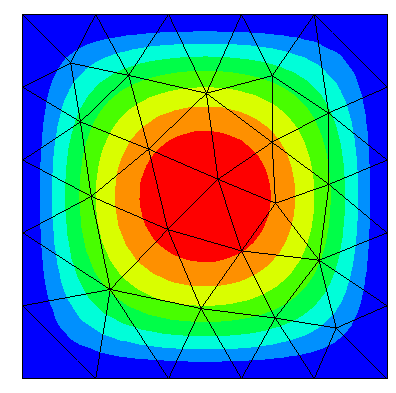
\includegraphics[scale=0.3]{../figures/mumps.png}
					\caption*{\tiny{Solution of Poisson problem computed with MUMPS}}
				\end{figure}
			\end{column}
		\end{columns}
	\end{frame}
	\begin{frame}[plain]
		\frametitle{PETSc KSP -- Iterative Jacobi method}
		\ngshead
		$\newline$
		$\newline$
		$\color{oxfordblue}\blacktriangleright$ We can use a wide variety of iterative solvers, for example, the Jacobi method, i.e.
		\begin{equation}
			x^{(k+1)} = D^{-1}(b - (A - D)x^{(k)}).
		\end{equation}
		\lstinputlisting[language=Python, firstline=52, lastline=58]{../examples/ngs/poisson.py.rst}
		$\newline$
		$\color{oxfordblue}\blacktriangleright$ Analogously we can implement the Gauss-Seidel method. 
	\end{frame}
	\begin{frame}[plain]
		\frametitle{PETSc KSP -- Galerkin Algebraic MultiGrid (GAMG)}
		\ngshead
		$\newline$
		$\newline$
		$\newline$
		$\color{oxfordblue}\blacktriangleright$ Inside of a classical iterative method such as conjugate gradient, we can play with different preconditioners such as PETSc GAMG.
		$\newline$
		\lstinputlisting[language=Python, firstline=61, lastline=64]{../examples/ngs/poisson.py.rst}
		$\newline$
		$\color{oxfordblue}\blacktriangleright$ As we will see in a moment we have a wide variety of preconditioners available, such as: \textbf{Hypre (AMG)}, \textbf{BDDC}, \textbf{...} 
	\end{frame}
	\begin{frame}[plain]
		\frametitle{An NGsolve Example -- Linear Elasticity}
		\ngshead
		$\newline$
		\lstinputlisting[language=Python, firstline=22, lastline=36]{../examples/ngs/elasticity.py.rst}
	\end{frame}
	\begin{frame}[plain]
		\frametitle{PETSc KSP -- Near Nullspace }
		$\newline$
		\ngshead
		$\newline$
		$\newline$
		$\color{oxfordblue}\blacktriangleright$ We can pass a near nullspace to a \textbf{KrylovSolver}, informing the solver that there is a near nullspace.
		\begin{columns}[T]
			\begin{column}{0.7\textwidth}
				\lstinputlisting[language=Python, firstline=41, lastline=49]{../examples/ngs/elasticity.py.rst}
			\end{column}
			\begin{column}{0.3\textwidth}
				\begin{figure}
					\centering
					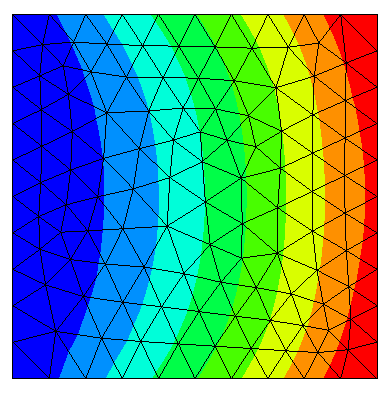
\includegraphics[scale=0.3]{../figures/nullspace.png}
					\caption*{\tiny{Solution of lienar elasticity fixing SO(3) to  be in the near nullspace.}}
				\end{figure}
			\end{column}
		\end{columns}
		\lstinputlisting[language=Python, firstline=50, lastline=51]{../examples/ngs/elasticity.py.rst}
	\end{frame}
	\section{\textbf{PETSc PC}}
	\begin{frame}[plain]
		\frametitle{PETSc PC -- Hypre}
		$\newline$
		\ngshead
		$\newline$
		$\newline$
		$\color{oxfordblue}\blacktriangleright$ We can use PETSc preconditioners as normal preconditioners in NGSolve, for example we can wrap a PETSc PC of type Hypre in NGSolve and use it inside NGSolve Krylov solvers.
		\lstinputlisting[language=Python, firstline=33, lastline=38]{../examples/ngs/precond.py.rst}
		\only<1>{
		\begin{center}
			\begin{tabular}{ |c||c|c|c|} 
			\hline
			Degrees of Freedom (p=1) &  7329 & 1837569 \\ 
			PETSc PC (HYPRE) & 22 (5.19e-13) & 31 (6.82e-13) \\ 
			NGSolve Geometric MultiGrid & 14 (4.08e-13) & 16 (1.30e-12)\\
			\hline
			\end{tabular}
		\end{center}
		}
		\only<2->{
		\begin{center}
			\begin{tabular}{ |c||c|c|c|} 
			\hline
			Degrees of Freedom (p=3) &  64993 & 259009  \\ 
			PETSc PC (HYPRE) & 40 (6.48e-13) & 69 (2.53e-13) \\ 
			NGSolve Geometric MultiGrid & 19 (8.89e-13) & 19 (7.78e-13)\\
			\hline
			\end{tabular}
		\end{center}
		}
	\end{frame}
	\begin{frame}[plain]
		\frametitle{PETSc PC -- Vertex Patch}
		$\newline$
		\ngshead
		$\newline$
		$\newline$
		$\color{oxfordblue}\blacktriangleright$ We can use PETSc preconditioner as one of the building blocks of a more complex preconditioner. For example, we can use it as a two-level additive Schwarz preconditioner.
		In this case, we will use as fine space correction, the inverse of the local matrices associated with the patch of a vertex, i.e.
		\begin{equation}
			\mathcal{P} = \sum_{i=1}^{n} I_i A_i^{-1}I_i^{T}.
		\end{equation}
		\vspace{-0.5cm}
		\lstinputlisting[language=Python, firstline=54, lastline=58]{../examples/ngs/precond.py.rst}
	\end{frame}
	\begin{frame}[plain]
		\frametitle{PETSc PC -- Two level additive Schwarz} 
		$\newline$
		\ngshead
		$\newline$
		$\newline$
		$\color{oxfordblue}\blacktriangleright$ We can also use the PETSc PC inside a two-level additive Schwarz preconditioner.
		In particular, we will use a PETSc PC of type HYPRE to do a coarse grid correction on the vertex degree of freedom. 
		\begin{equation}
			\mathcal{P} = I_{H}A_{H}^{-1}I_{H}^{T} + \sum_{i=1}^{n} I_i A_i^{-1}I_i^{T}.
		\end{equation}
		\vspace{-0.5cm}
		\lstinputlisting[language=Python, firstline=70, lastline=73]{../examples/ngs/precond.py.rst}
	\end{frame}
	\begin{frame}[plain]
		\frametitle{An NGsolve Example -- Discontinuous Galerkin}
		$\newline$
		$\newline$
		\ngshead
		\lstinputlisting[language=Python, firstline=79, lastline=98]{../examples/ngs/precond.py.rst}
	\end{frame}
	\begin{frame}[plain]
		\frametitle{PETSc PC -- Auxiliary Space Preconditioner}
		$\newline$
		\ngshead
		$\newline$
		$\newline$
		$\color{oxfordblue}\blacktriangleright$ 
		We can now use the PETSc PC assembled for the conforming Poisson problem as an auxiliary space preconditioner for the DG discretisation.
		In particular, we will use as smoother a PETSc PC of type SOR.
		$\newline$
		\lstinputlisting[language=Python, firstline=101, lastline=106]{../examples/ngs/precond.py.rst}
	\end{frame}
	\section{\textbf{Saddle Point Problems}}
	\begin{frame}[plain]
		\frametitle{An NGsolve Example -- Stokes flow}
		$\newline$
		$\newline$
		\ngshead
		$\newline$
		\lstinputlisting[language=Python, firstline=30, lastline=39]{../examples/ngs/saddle.py.rst}
		\begin{figure}
			\centering
			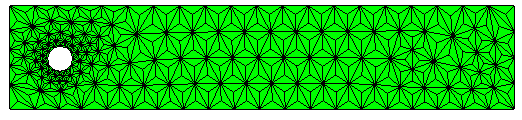
\includegraphics[scale=0.4]{../figures/channel.png}
		\end{figure}
	\end{frame}
	\begin{frame}
		\frametitle{Fieldsplit Schur preconditioner -- Mass matrix}
		$\newline$
		$\newline$
		It is well known that a field split preconditioner can be used to solve saddle point problems, i.e.
		\begin{equation}
			\begin{bmatrix}
				\hat{A}^{-1}& 0\\
				0 & -B\hat{A}^{-1}B^T
			\end{bmatrix}
		\end{equation}
		Thanks to the inf-sup condition we can prove that the Schur complement is spectrally equivalent to the mass matrix, hence we can use as preconditioner:
		\vspace{-0.2cm}
		\begin{equation}
			\begin{bmatrix}
				\hat{A}^{-1}& 0\\
				0 & -\nu \hat{M}^{-1}
			\end{bmatrix}
		\end{equation}
		where $M$ is the mass matrix.
	\end{frame}
	\begin{frame}[plain]
		\frametitle{PETSc PC -- NGSolve Fieldsplit}
		$\newline$
		$\newline$
		\ngshead
		$\newline$
		\lstinputlisting[language=Python, firstline=43, lastline=53]{../examples/ngs/saddle.py.rst}
		\begin{figure}
			\centering
			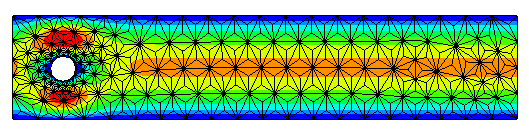
\includegraphics[scale=0.4]{../figures/stokes.png}
		\end{figure}
	\end{frame}
	%\begin{frame}{Navier-Stokes flow}
	%	A more interesting example is the Navier-Stokes flow, which is a non-linear problem.
	%	In particular, we will consider the problem of finding $(\vec{u},p) \in H^1(\Omega)^2\times L^2(\Omega)$ such that
	%	\begin{align*}
	%		\int_\Omega \partial_t \vec{u} \cdot \vec{v} + \int_\Omega(\vec{u}\cdot \nabla) \vec{u}\cdot\vec{v}+\nu\int_{\Omega} \nabla \vec{u} : \nabla \vec{v} - \int_{\Omega} p \nabla \cdot \vec{v} &= \int_{\Omega} \vec{f} \cdot \vec{v}\\
	%		-\int_{\Omega} q \nabla \cdot \vec{u} &= 0
	%	\end{align*}
	%	for all $(\vec{v},q) \in H^1(\Omega)^2\times L^2(\Omega)$.
	%\end{frame}
	%\begin{frame}{Navier-Stokes flow -- Augmented Lagrangian}
	%	$\newline$
	%	We consider an augmented Lagrangian formulation for the discrete problem, i.e. find $(\vec{u}_h,p_h) \in V_h \times Q_h$ such that
	%	\begin{align*}
	%		(\partial_t\vec{u},\vec{v})_0 + (\vec{u}\cdot \nabla \vec{u},\vec{v})_0 &+ \nu(\nabla \vec{u},\nabla \vec{v})_0 \\
	%		 & - (p,\nabla \cdot \vec{v})_0 + \gamma(\nabla \cdot \vec{u},\nabla \cdot \vec{v})_0 &= (\vec{f},\vec{v})_0\\
	%	\end{align*}
	%	and verifying the weak divergence free constraint $(\nabla \cdot \vec{u},q)_0 = 0$, for all $(\vec{v},q) \in V_h \times Q_h$.
	%\end{frame}
	%\begin{frame}
	%	\frametitle{Navier-Stokes flow -- Fieldsplit Schour preconditioner}
	%	$\newline$
	%	$\newline$
	%	The linearized version of the Navier-Stokes equations can be written in matrix form as 
	%	\vspace{-0.1cm}
	%	\begin{equation}
	%		\begin{bmatrix}
	%			A+\gamma B^TWB& B^T \\
	%			B & 0
	%		\end{bmatrix}
	%		\begin{bmatrix}\vec{u} \\p\end{bmatrix}=\begin{bmatrix}\vec{f} \\0\end{bmatrix}
	%	\end{equation}
	%	We choose as preconditioner the \textbf{fieldsplit Schur preconditioner}, i.e.
	%	\vspace{-0.1cm}
	%	\begin{equation}
	%		\begin{bmatrix}
	%			I & -\hat{A}_\gamma^{-1} B^T\\
	%			0 & I
	%		\end{bmatrix}
	%		\begin{bmatrix}
	%			\hat{A}_\gamma^{-1}& 0\\
	%			0 & \hat{S}_\gamma^{-1}
	%		\end{bmatrix}
	%		\begin{bmatrix}
	%			I & 0\\
	%			-BA_\gamma^{-1} & I
	%		\end{bmatrix}
	%	\end{equation}
	%	\begin{equation}
	%		A_\gamma = A+\gamma B^TWB 	\qquad  S_\gamma = -BA_\gamma^{-1}B^T.
	%	\end{equation}
	%\end{frame}
	%\begin{frame}{Navier-Stokes flow -- Augmented Lagrangian}
	%	$\newline$
	%	\begin{itemize}
	%		\item [\color{oxfordblue}$\blacktriangleright$] The augmented Lagrangian term helps enforce the divergence-free constraint, and makes the scheme pressure robust.
	%		\item [\color{oxfordblue}$\blacktriangleright$] We can use as preconditioner
	%		\begin{equation}
	%			\begin{bmatrix}
	%				\hat{A}_\gamma^{-1}& 0\\
	%				0 & -(\nu+\gamma)M^{-1}
	%			\end{bmatrix}
	%		\end{equation}
	%		\item[\color{oxfordblue}$\blacktriangleright$] How do we compute $\hat{A}_\gamma^{-1}$ efficiently ? Can we adopt a multigrid approach ?
	%	\end{itemize}
	%\end{frame}
	%\begin{frame}[fragile]
	%	\frametitle{Robust relaxation via FEEC -- Hood--Taylor}
	%	\begin{equation*}
	%		\begin{tikzcd}[row sep=huge]
	%		0 \arrow[r,""] & \Big[H^2(\Omega)\Big]^2 \arrow[r,"\curl"] \arrow[d]& \Big[H^1_0(\Omega)\Big]^2 \arrow[r,"\div"] \arrow[d]& L^2(\Omega) \arrow[r,""]\arrow[d] & 0\\
	%		0 \arrow[r,""] & \Big[\mathbb{P}^5(\mathcal{T}_h)\Big]^2 \arrow[r,"\curl"] & \Big[\mathbb{P}^4(\mathcal{T}_h)\Big]^2 \arrow[r,"\div"] & \mathbb{P}^3_{disc}(\mathcal{T}_h) \arrow[r,""] & 0\\
	%		\end{tikzcd}
	%	\vspace{-1cm}
	%	\end{equation*}
	%	$\color{oxfordblue}\blacktriangleright$ Thanks to the FEEC complex we can construct a robust relaxation and prolongation operator for the Hood--Taylor element.
	%\end{frame}
	\section{\textbf{PETSc SNES}}
	\begin{frame}[plain]
		\frametitle{An NGsolve Example -- Naghdi Shell}
		$\newline$
		$\newline$
		\ngshead
		$\newline$
		\begin{columns}[T]
			\begin{column}{0.7\textwidth}
				\lstinputlisting[language=Python, firstline=9, lastline=21]{../examples/ngs/legacy/naghdi.py}
			\end{column}
			\begin{column}{0.25\textwidth}
				\begin{figure}
					\centering
					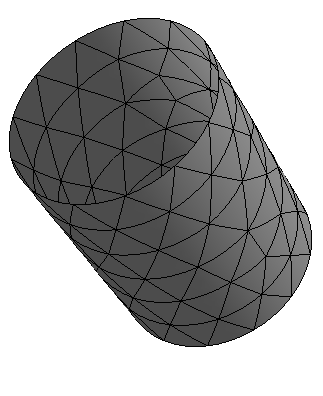
\includegraphics[scale=0.3]{../figures/shell.png}
					\caption*{\tiny{Naghdi shell undeformed geometry.}}
				\end{figure}
			\end{column}
		\end{columns}
	\end{frame}
	\begin{frame}[plain]
		\frametitle{An NGsolve Example -- Naghdi Shell}
		$\newline$
		$\newline$
		\ngshead
		\lstinputlisting[language=Python, firstline=27, lastline=43]{../examples/ngs/legacy/naghdi.py}
	\end{frame}
	\begin{frame}[plain]
		\frametitle{PETSc SNES}
		\ngshead
		$\newline$
		$\newline$
		$\newline$
		$\color{oxfordblue}\blacktriangleright$ We can use PETSc SNES to solve the non-linear Naghdi shell problem.
		$\newline$
		\begin{columns}[T]
			\begin{column}{0.7\textwidth}
				\lstinputlisting[language=Python, firstline=49, lastline=56]{../examples/ngs/legacy/naghdi.py}
			\end{column}
			\begin{column}{0.3\textwidth}
				\vspace{-0.8cm}
				\begin{figure}
					\centering
					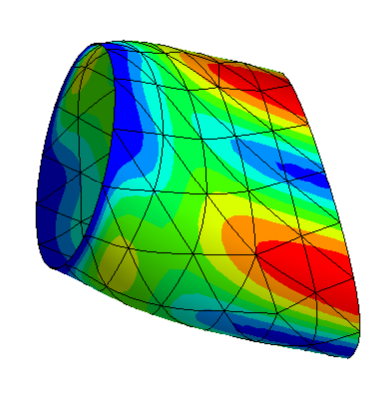
\includegraphics[scale=0.3]{../figures/naghdi.png}
					\caption*{\tiny{Solution of Naghdi shell problem.}}
				\end{figure}
			\end{column}
		\end{columns}
	\end{frame}
	\section{\textbf{PETSc DMPLEX}}
	\begin{frame}[plain]
		\firedrakehead
		$\newline$
		$\newline$
		\textbf{Firedrake} is an automated system for the solution of partial differential equations using the finite element method (FEM).
		$\newline$
		$\newline$
			\begin{itemize}
				\item[\color{oxfordblue}$\blacktriangleright$] Variational formulation can be easily defined using the \textbf{UFL} language.
				\item[\color{oxfordblue}$\blacktriangleright$] Wide class of finite elements are available, including $H(div)$, $H(curl)$, $H^1$ and $H^2$.
				\item[\color{oxfordblue}$\blacktriangleright$] Provides access to \textbf{PETSc} linear solvers and non-linear solvers.
			\end{itemize}
	\end{frame}
	\begin{frame}
		\frametitle{ngsPETSc -- Firedrake}
		$\newline$
		\textbf{ngsPETSc} provides new capabilities to \textbf{Firedrake} such as:
		$\newline$
		\begin{itemize}
			\item[\color{oxfordblue}$\blacktriangleright$] Access to all Netgen generated linear meshes and high order meshes.
			\item[\color{oxfordblue}$\blacktriangleright$] Splits for macro elements, such as Alfeld splits and Powell-Sabin splits (even on curved geometries).
			\item[\color{oxfordblue}$\blacktriangleright$] Adaptive mesh refinement capabilities, that conform to the geometry.
			\item[\color{oxfordblue}$\blacktriangleright$] High order mesh hierarchies for multigrid solvers. 
		\end{itemize}
	\end{frame}
	\section{\textbf{SLEPc EPS}}
	\begin{frame}[plain]
		\frametitle{An NGsolve Example -- Mass conserving scheme}
		$\newline$
		$\newline$
		\ngshead
	\lstinputlisting[language=Python, firstline=36, lastline=55]{../examples/ngs/legacy/MCSEig.py}
	\end{frame}
	\begin{frame}[plain]
		\frametitle{SLEPc ESP}
		$\newline$
		\ngshead
		$\newline$
		$\newline$
		$\color{oxfordblue}\blacktriangleright$ We easily solve the eigenvalue problem associated to the Stokes formulation using ngsPETSc EigenSolver.
		\begin{columns}[T]
			\begin{column}{0.7\textwidth}
				\lstinputlisting[language=Python, firstline=59, lastline=69]{../examples/ngs/legacy/MCSEig.py}
			\end{column}
			\begin{column}{0.3\textwidth}
				\begin{figure}
					\centering
					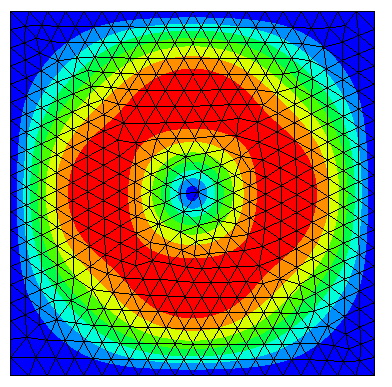
\includegraphics[scale=0.3]{../figures/eig.png}
					\caption*{\tiny{First eigenfunctions of the Stokes eigenvalue problem}}
				\end{figure}
			\end{column}
		\end{columns}
	\end{frame}
	\section{\textbf{Conclusions}}
	\begin{frame}
		\frametitle{Future developments}
		\begin{itemize}
			\item [$\color{oxfordblue}\blacktriangleright$] We plan to extend the interface to include time-stepping capabilities from \textbf{PETSc TS}.
			\item [$\color{oxfordblue}\blacktriangleright$] We plan to expriment with \textbf{HPDDM}.
			\item [$\color{oxfordblue}\blacktriangleright$] We plan to use \textbf{PETSc} as linear algebra backend in \textbf{NGSolve} to ensure cross-architecture compatibility and GPU acceleration.
		\end{itemize}
	\end{frame}
	\begin{frame}{NGSolve User Meeting}
		$\newline$
		$\newline$
		$\color{oxfordblue}\blacktriangleright$ Come to the 5th NGSolve User Meeting that will be held between the \textbf{17th of June} and the \textbf{19th of June} at \textbf{TU Wien}.
		\begin{figure}
			\centering
			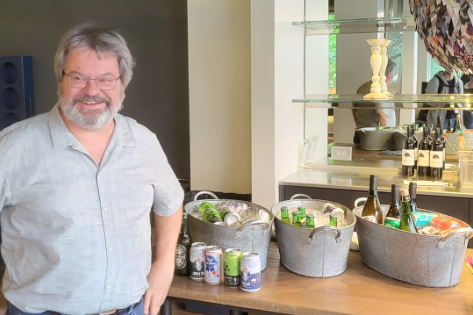
\includegraphics[scale=0.5]{../figures/joachim.png}
		\end{figure}
		\vspace{-0.6cm}
		\begin{center}
			\textbf{Usally there are beers !}
		\end{center}
	\end{frame}
\end{document}
